\section{Adaptive AR Model Based Time-Frequency Estimation}
\subsection{AR modelling of FM signal}
\begin{figure}[htb]
	\centering
    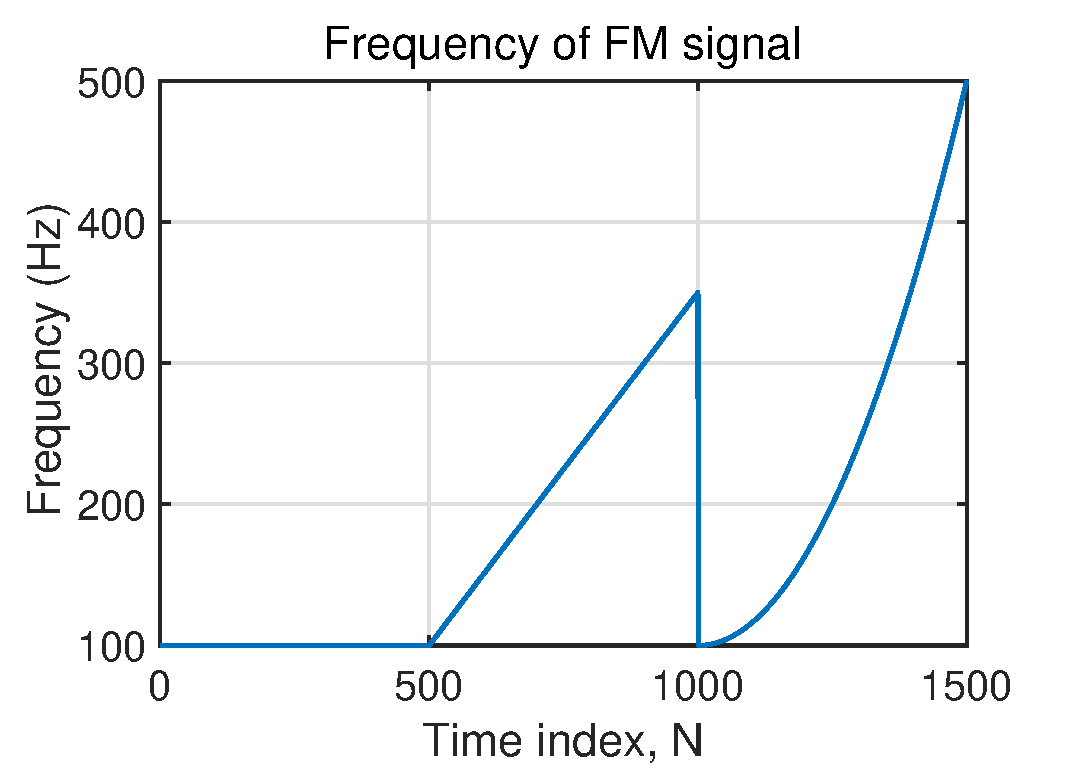
\includegraphics[width=0.36\textwidth]{fig/32/32a1.eps}
    \caption{Time-variant frequency of FM signal}
    \label{fig:3_2_a1}
\end{figure}
\noindent
A FM signal with time-variant frequency as shown in Fig.\ref{fig:3_2_a1} is modulated with adding white noise in distribution of $\mathcal N\in$ (0, 0.05). The frequency is composed of three segments with constant, linear and quadratic parts, resulting in the non-stationary FM signal.
\begin{figure}[htb]
     \centering
     \hspace{-0.4cm}
     \begin{subfigure}[b]{0.33\textwidth}
         \centering
         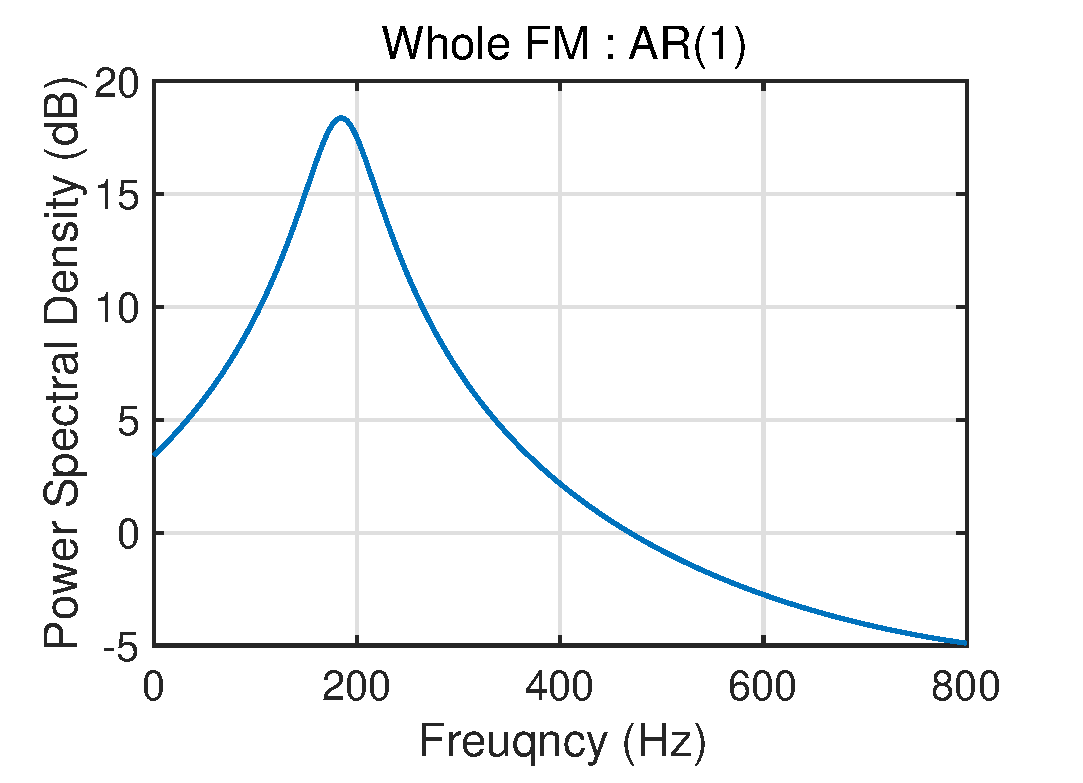
\includegraphics[width=\textwidth]{fig/32/32a2.eps}
     \end{subfigure}
    \hspace{-0.4cm}
     \begin{subfigure}[b]{0.33\textwidth}
         \centering
         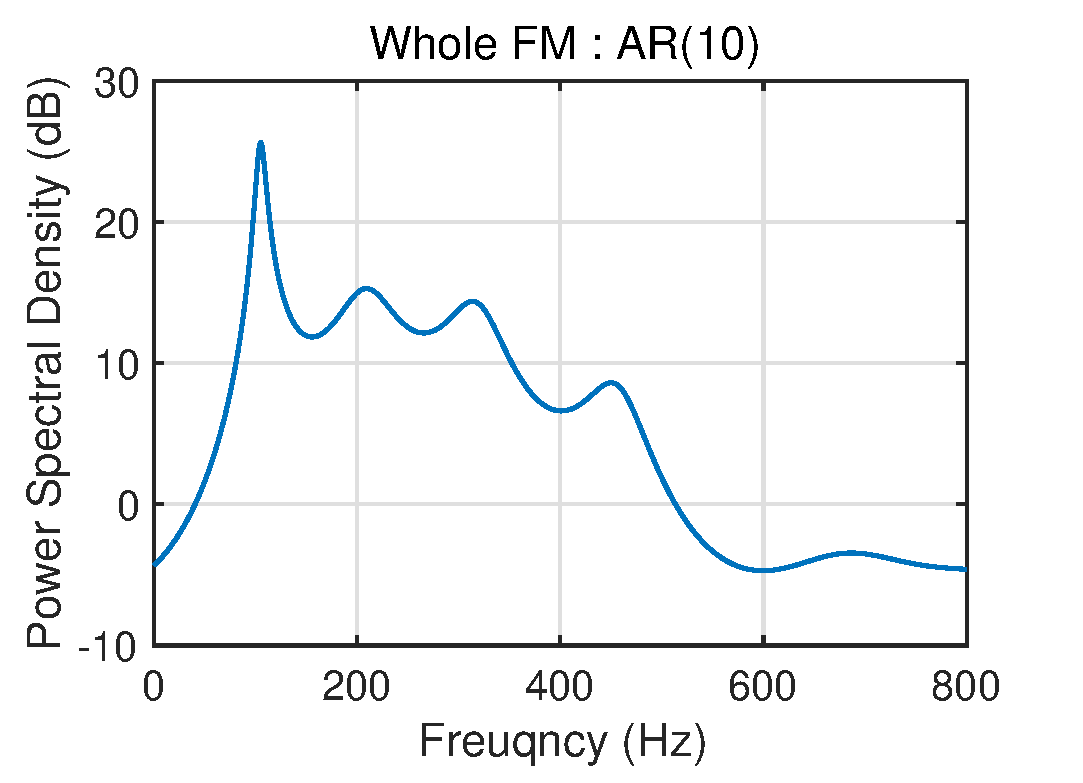
\includegraphics[width=\textwidth]{fig/32/32a3.eps}
     \end{subfigure}
    \hspace{-0.4cm}
     \begin{subfigure}[b]{0.33\textwidth}
         \centering
         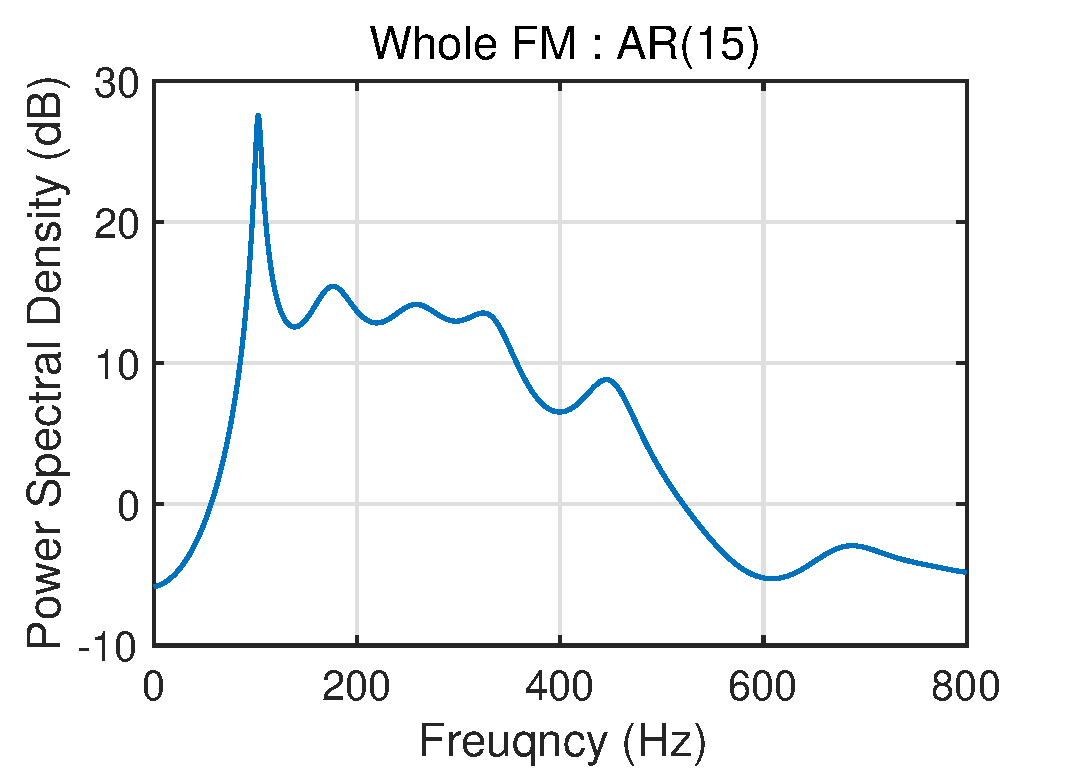
\includegraphics[width=\textwidth]{fig/32/32a4.eps}
     \end{subfigure}
    \caption{Whole FM AR estimation with order=1, 10 and 15}
    \label{fig:3_2_a2}
\end{figure}\\
When using the MATLAB function \texttt{aryule} to estimate the coefficient for entire signal, Fig.\ref{fig:3_2_a2} depicts the performance of estimations with different orders. For AR(1) modelling, the estimated peak of frequency is inaccurate since the function is incapable to estimate non-stationary signal. With increasing the order of estimated model, only the constant frequency at $100Hz$ is successfully estimated. However, other segments frequencies are still not captured accurately. Thus, the previous method in Part 2.2 is not applicable for FM signal.
\begin{figure}[htb]
     \centering
     \hspace{-0.4cm}
     \begin{subfigure}[b]{0.32\textwidth}
         \centering
         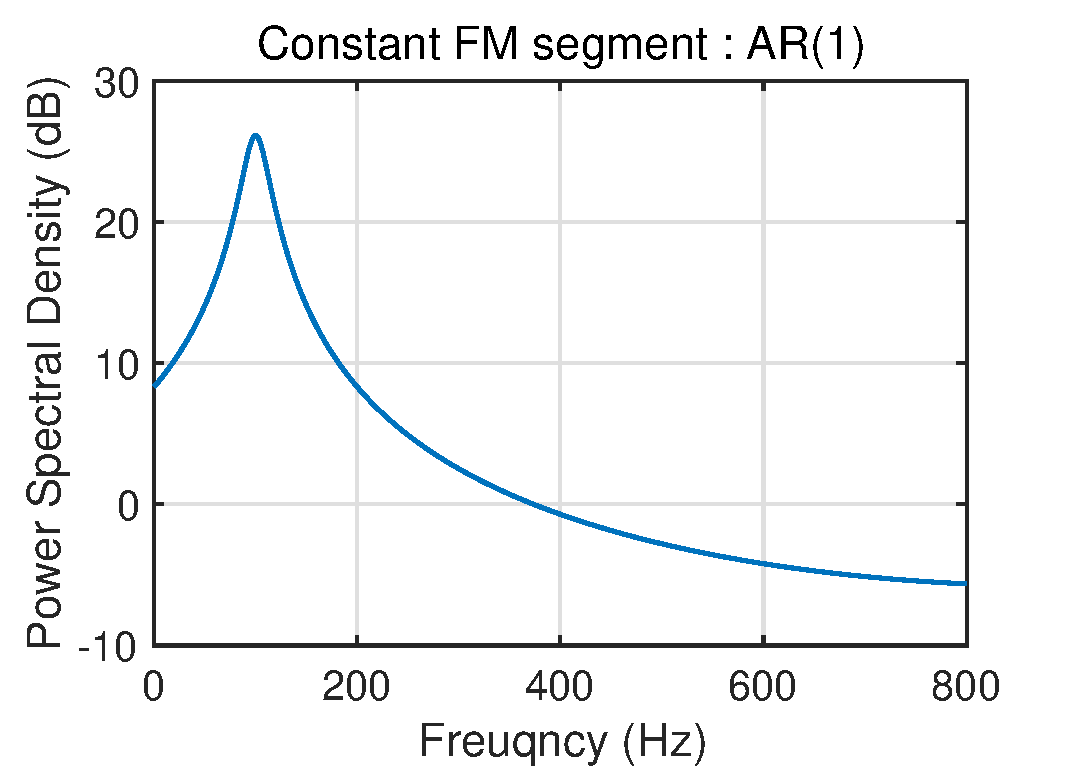
\includegraphics[width=\textwidth]{fig/32/32a5.eps}
     \end{subfigure}
    \hspace{-0.4cm}
     \begin{subfigure}[b]{0.32\textwidth}
         \centering
         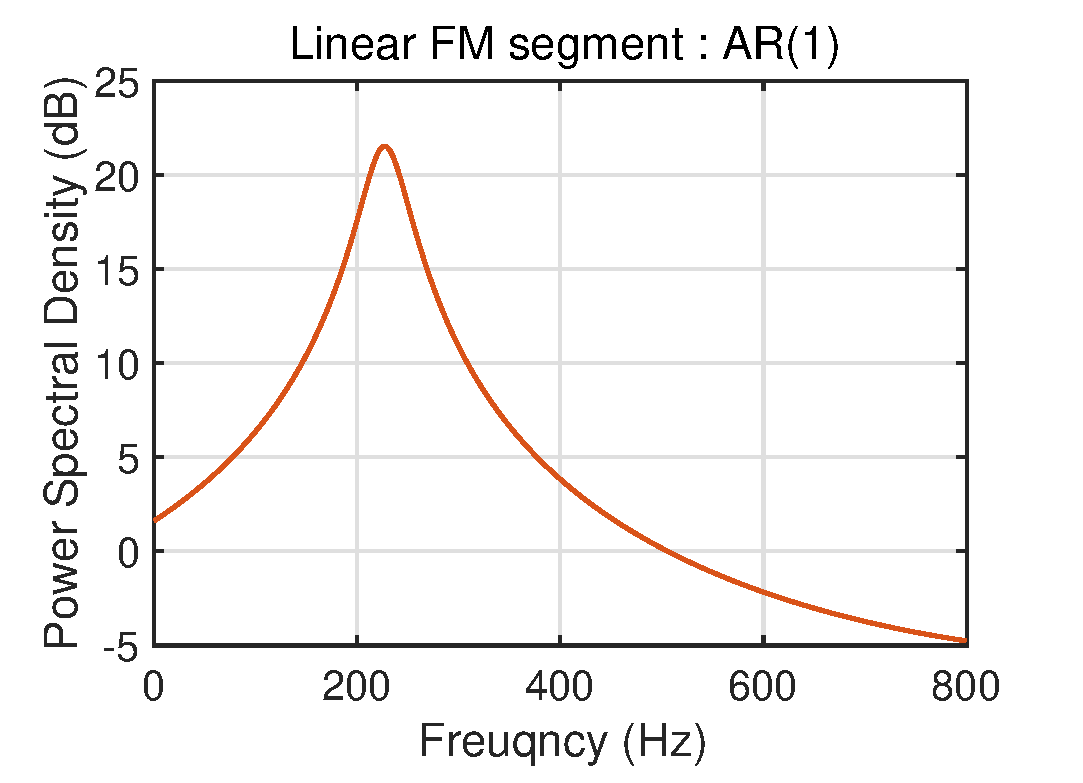
\includegraphics[width=\textwidth]{fig/32/32a6.eps}
     \end{subfigure}
    \hspace{-0.4cm}
     \begin{subfigure}[b]{0.32\textwidth}
         \centering
         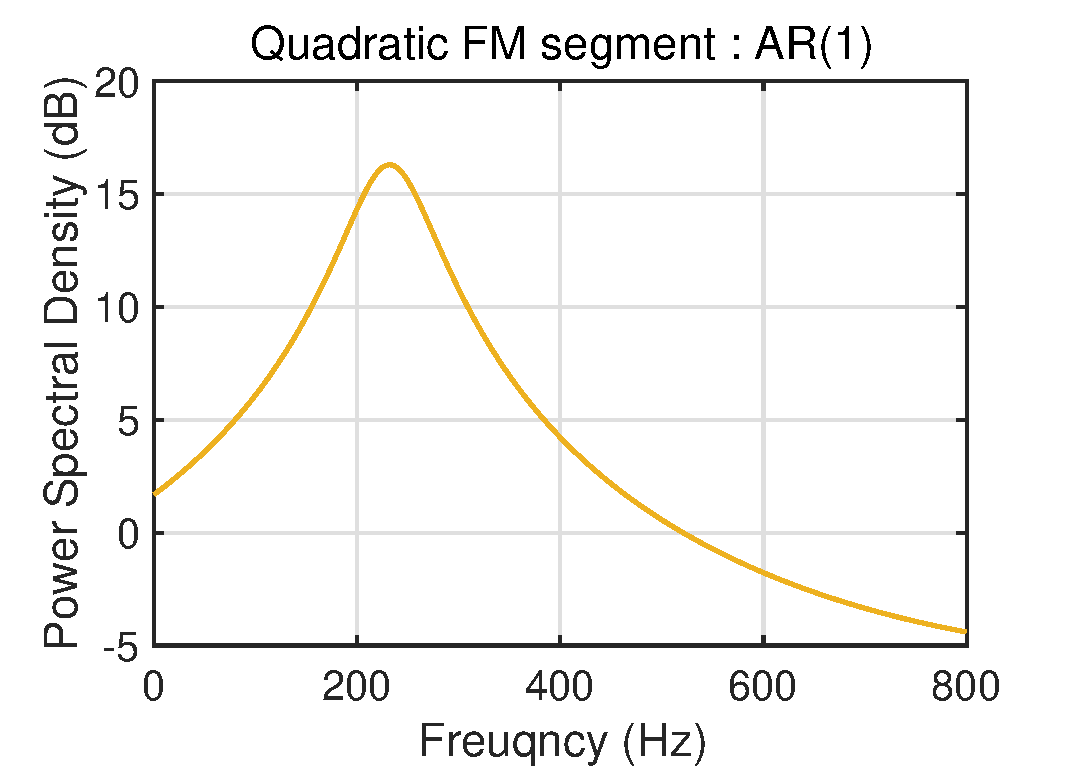
\includegraphics[width=\textwidth]{fig/32/32a7.eps}
     \end{subfigure}
     \\
     \hspace{-0.4cm}
     \begin{subfigure}[b]{0.32\textwidth}
         \centering
         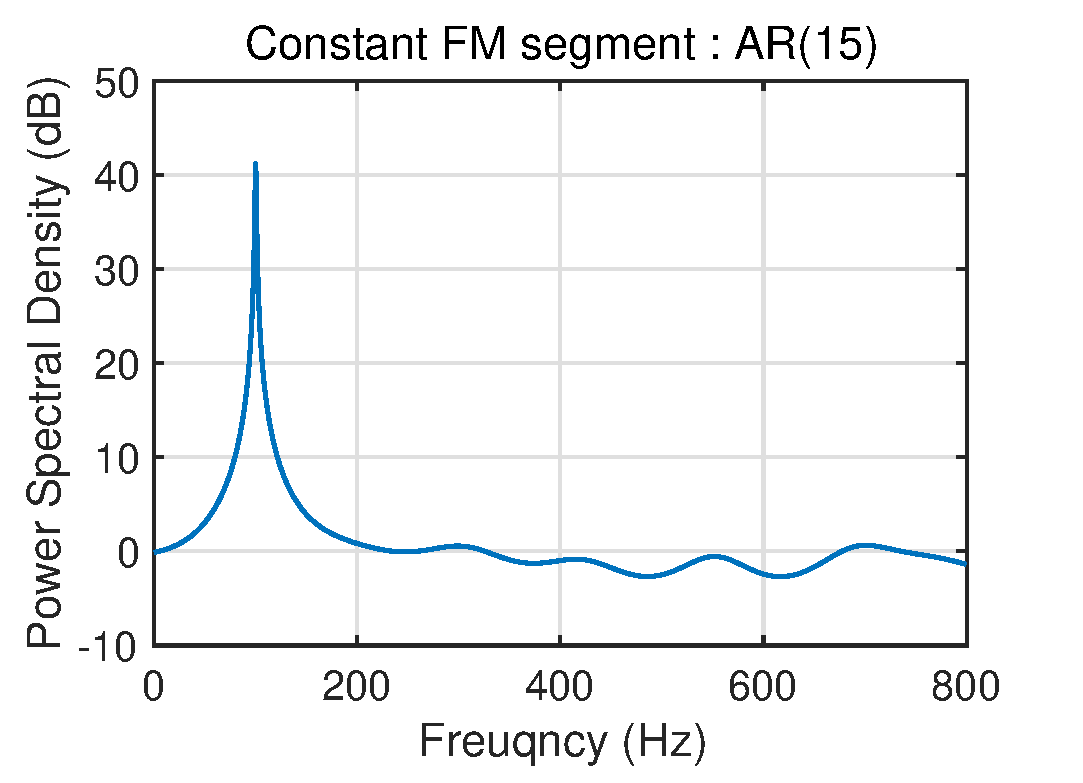
\includegraphics[width=\textwidth]{fig/32/32a8.eps}
     \end{subfigure}
    \hspace{-0.4cm}
     \begin{subfigure}[b]{0.32\textwidth}
         \centering
         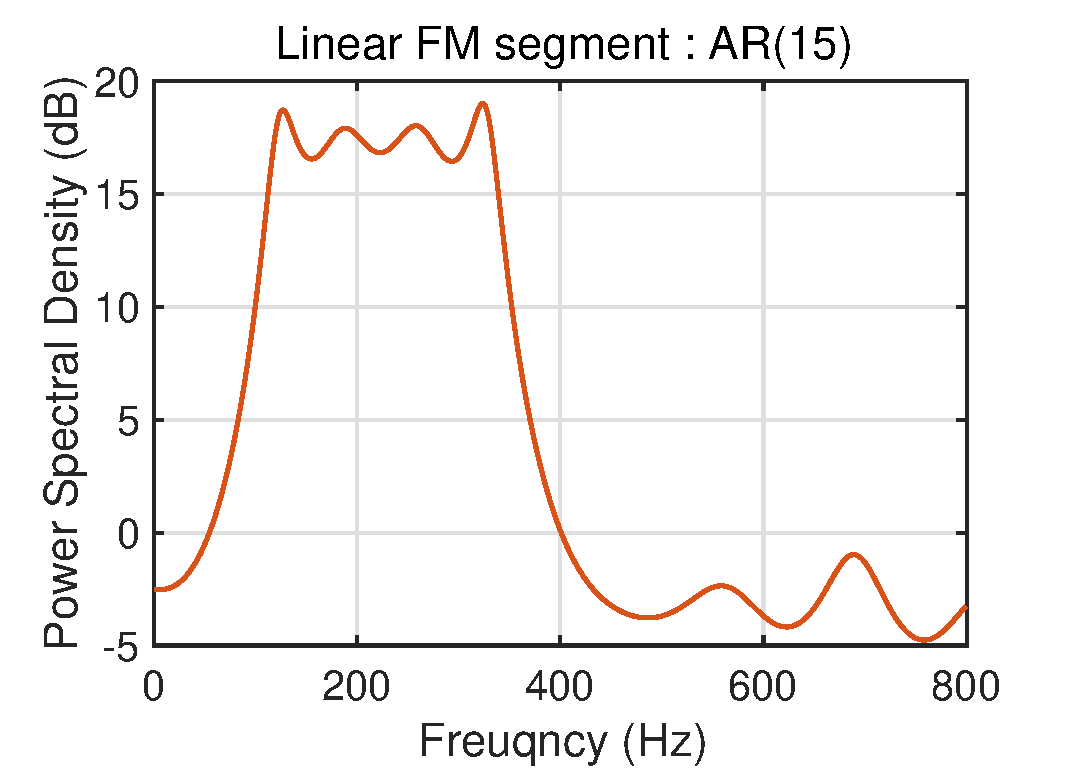
\includegraphics[width=\textwidth]{fig/32/32a9.eps}
     \end{subfigure}
    \hspace{-0.4cm}
     \begin{subfigure}[b]{0.32\textwidth}
         \centering
         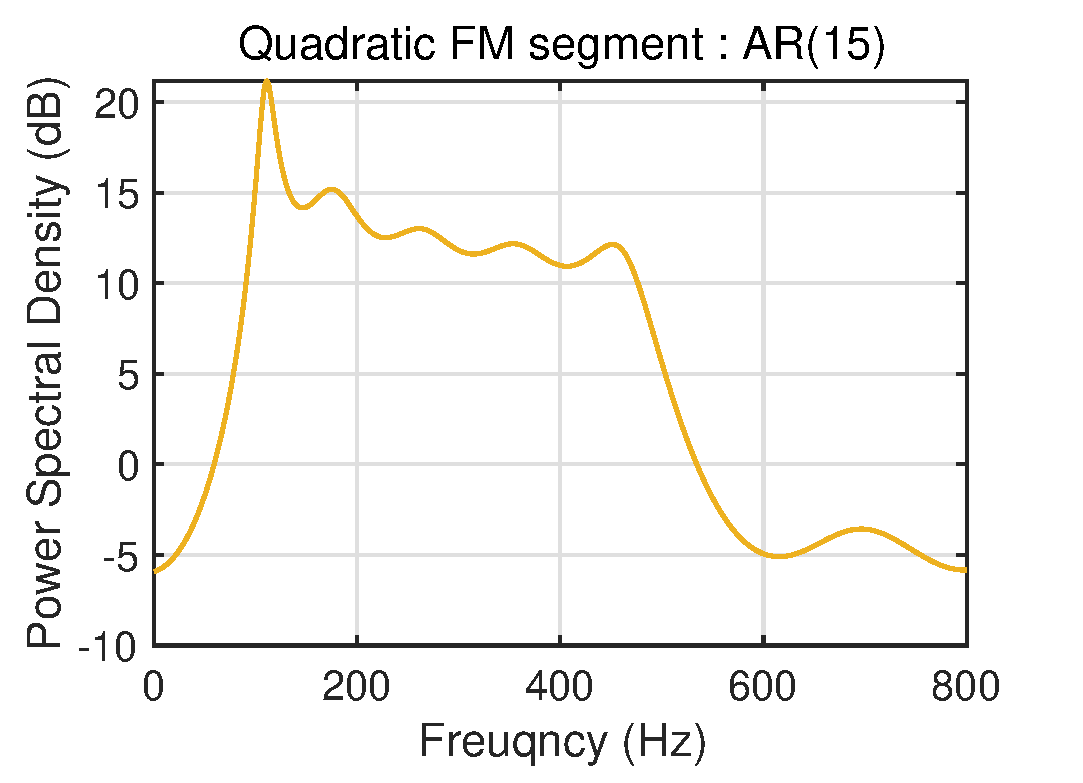
\includegraphics[width=\textwidth]{fig/32/32a10.eps}
     \end{subfigure}
        \caption{Block-based AR estimation with order=1 and 15}
        \label{fig:3_2_a3}
\end{figure}\\
In addition, the frequency is time-varying function with constant, linear and quadratic segments. Thus, the block-based estimation is implemented with segments length $N=500$ samples. Fig.\ref{fig:3_2_a3} illustrates the performance of estimated AR model with order 1 and 15. The constant frequency part can be successfully estimated with $p=1$ presented in a peak value at $100Hz$. However, the linear and quadratic segments perform inferior with inaccurate frequencies. By increasing the capacity of estimated model, the frequency range of segment can be approximately estimated with acceptable uncertainty, as shown in second row of Fig.\ref{fig:3_2_a3}. Nevertheless, the linear and quadratic relationship can not be observed based on the estimation since they are not satisfied with stationary.
\subsection{CLMS based estimated AR coefficient}
In this section, the CLMS algorithm is applied to estimate non-stationary signal. Fig.\ref{fig:3_2_b} shows the performance of estimating AR(1) coefficients with varying step-size $\mu$. It is obviously that the CLMS can adaptively capture the time-variant frequencies. However, the different step-size $\mu$ also affects the performance of the CLMS estimation. With small step-size, the learning curve can not converge, leading to inadequate estimation. The performance at $\mu=0.01$ is improved in spite of lacking beginning parts of the constant frequency. Setting $\mu=0.05$ introduces an optimal estimation, while larger step causes oscillation in convergence. As a consequence, there are large variance and distortions of spectrum.
\begin{figure}[htb]
     \centering
     \hspace{0.4cm}
     \begin{subfigure}[b]{0.35\textwidth}
         \centering
         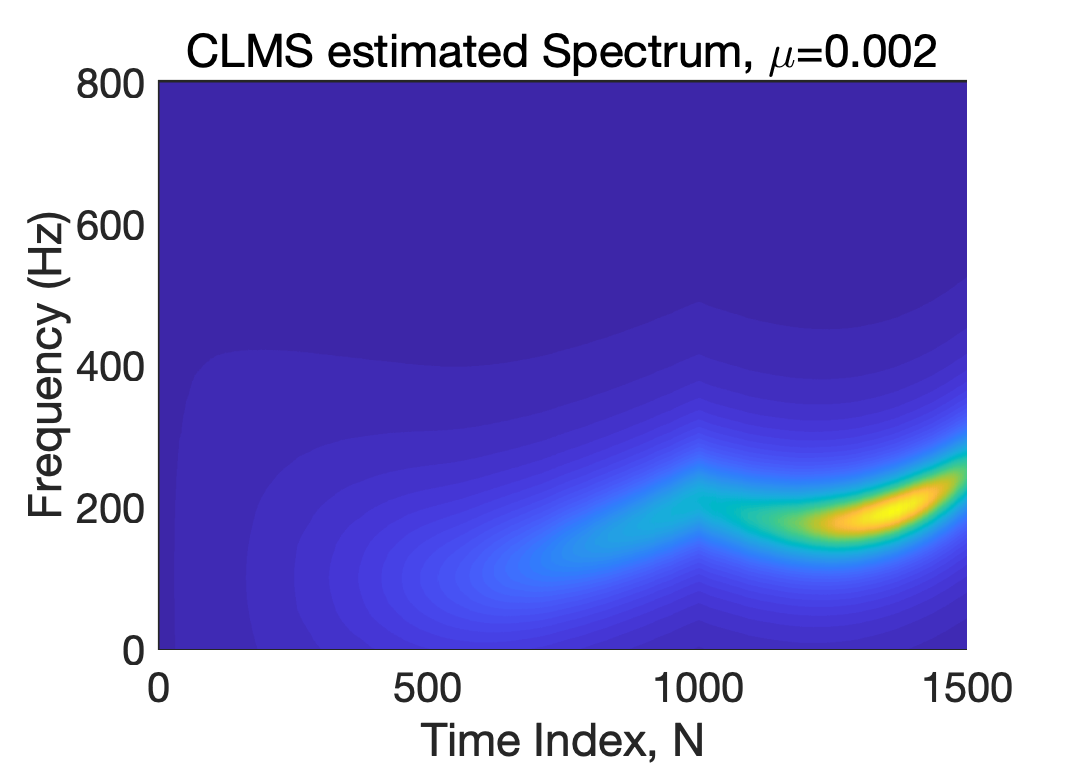
\includegraphics[width=\textwidth]{fig/32/32b1.eps}
     \end{subfigure}
    \hspace{0.4cm}
     \begin{subfigure}[b]{0.35\textwidth}
         \centering
         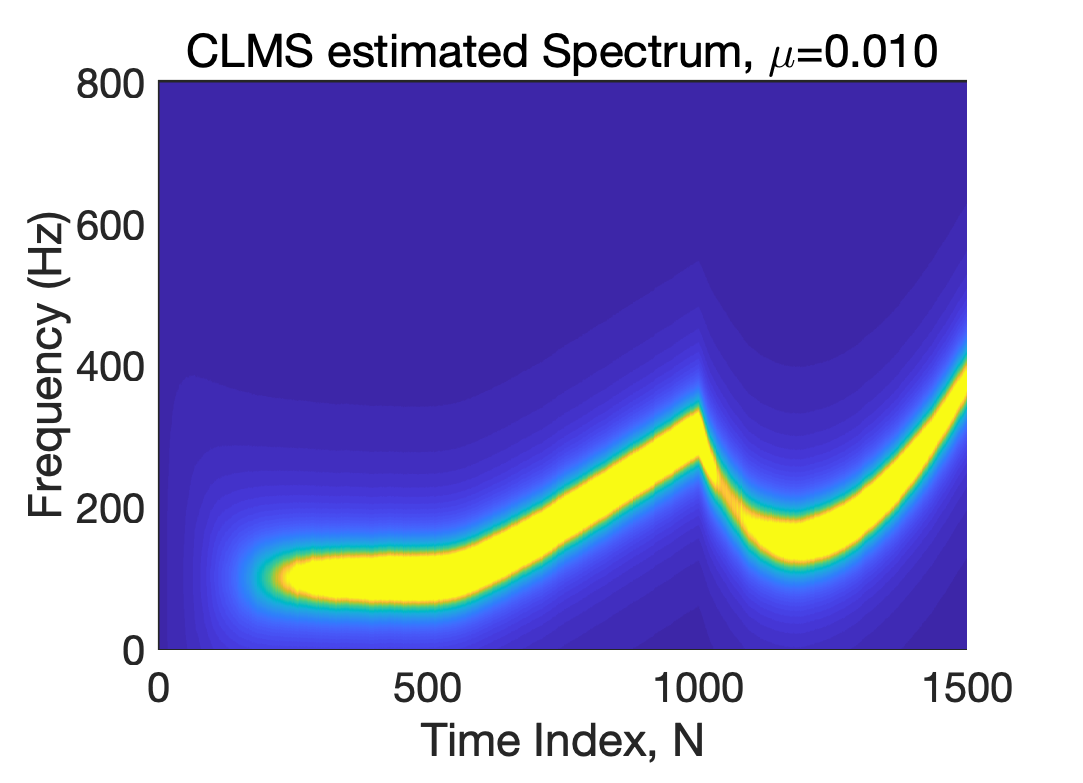
\includegraphics[width=\textwidth]{fig/32/32b2.eps}
     \end{subfigure}
    \\
    \hspace{0.4cm}
     \begin{subfigure}[b]{0.35\textwidth}
         \centering
         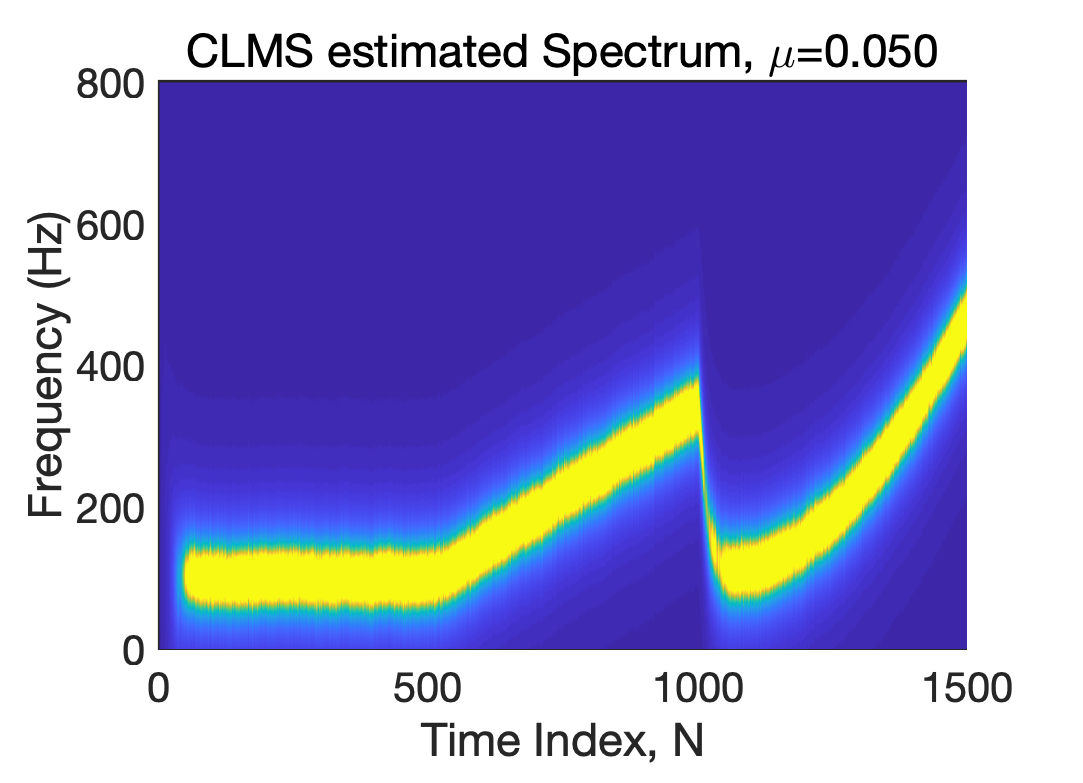
\includegraphics[width=\textwidth]{fig/32/32b3.eps}
     \end{subfigure}
     \hspace{0.4cm}
     \begin{subfigure}[b]{0.35\textwidth}
         \centering
         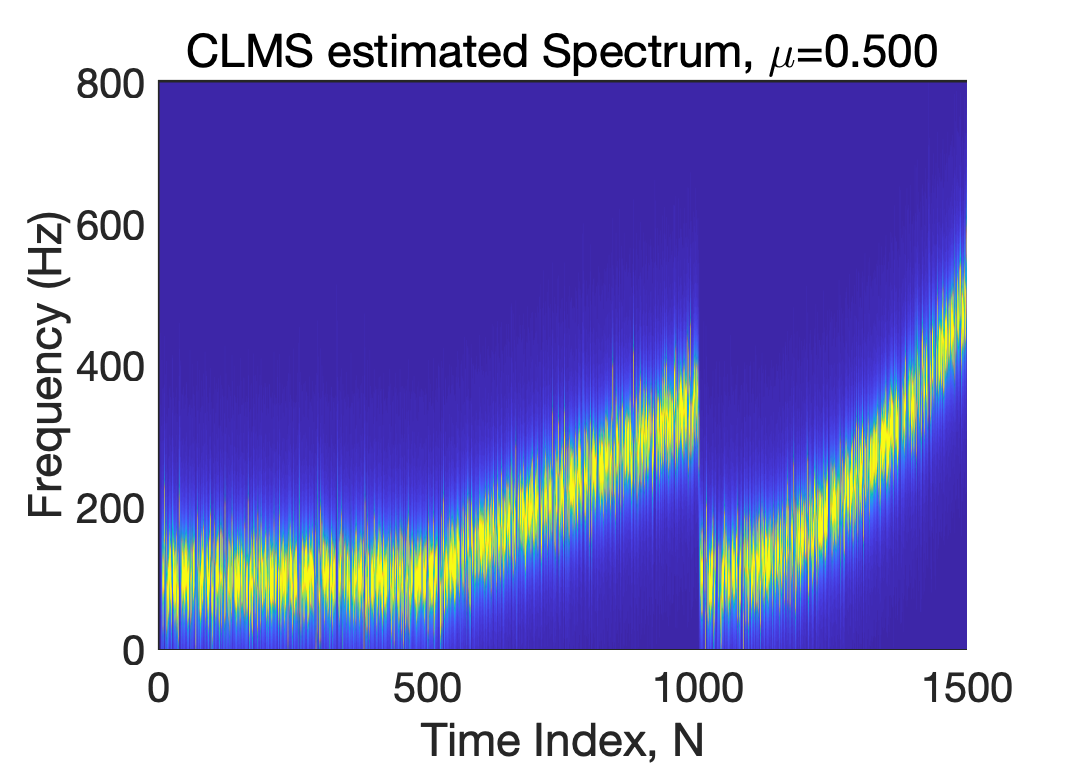
\includegraphics[width=\textwidth]{fig/32/32b4.eps}
     \end{subfigure}
        \caption{CLMS-based AR estimation with different step $\mu$}
        \label{fig:3_2_b}
\end{figure}
